\chapter{Evaluation}\label{ch:Evaluation}
In this chapter, the produced artefact will be evaluated against its original requirements.
In addition, the development process itself will be reflected upon to identify where issues arose 
and could have been prevented.

\section{Product}
% Within Section \ref{sec:Requirements}, the functional and non-functional requirements for this project were stated.
% Of these requirements, the chatbot successfully meets all functional requirements, as well as the original aims and 
% objectives stated in \ref{sec:AimsAndObjectives}. However, two non-functional requirements were not met.

% \para One of these requirements was 'The chatbot could allow for voice input and output.' This requirement was not met,
% as it would introduce a significant cost and time investment in trying to integrate this functionality into a Streamlit 
% web app. The other unmet requirement was 'The chatbot could be deployed on an existing messaging service.' This requirement 
% was not met due to time constraints, which is further reflected upon in Section \ref{sec:EvalProcess}. 

\para To properly evaluate the chatbot, it is best to use direct evaluation metrics. While reviewing literature in Section 
\ref{sec:LitReviewLLM}, an evaluation platform known as DeepEval was considered, with the ability to use an LLM as a judge of 
other LLMs \autocite{deepeval_introduction_2024}, known as 'G-Eval'.

\subsection{G-Eval}\label{sec:DeepEval}
DeepEval offers a wide variety of metrics, with one of these metrics being 'GEval'. GEval is a metric which is scored by an LLM based 
on criteria given in natural language, originally created by \textcite{liuGEvalNLGEvaluation2023a}. This means that the metric is directly 
programmable using a system prompt as seen with the chatbot itself.

\para 
To evaluate the chatbot, an evaluation dataset of questions and their expected answers was provided, with the chatbot's actual response being
compared to the expected answer which is known to be true (referred to as a 'golden answer'.). It is common practice when using G-Eval to use a 
superior LLM for evaluation than the one that originally generated the answer. Therefore, for G-Eval, gpt-4o was used, making the evaluation process 
the most expensive part of this project. 

\para A dataset of 10 questions was created with expected answers. DeepEval provides an 'LLMTestCase' class allowing for these to be neatly 
organised, as depicted in Figure \ref{fig:TestCaseCode}.

\begin{figure}[H]
    \centering
    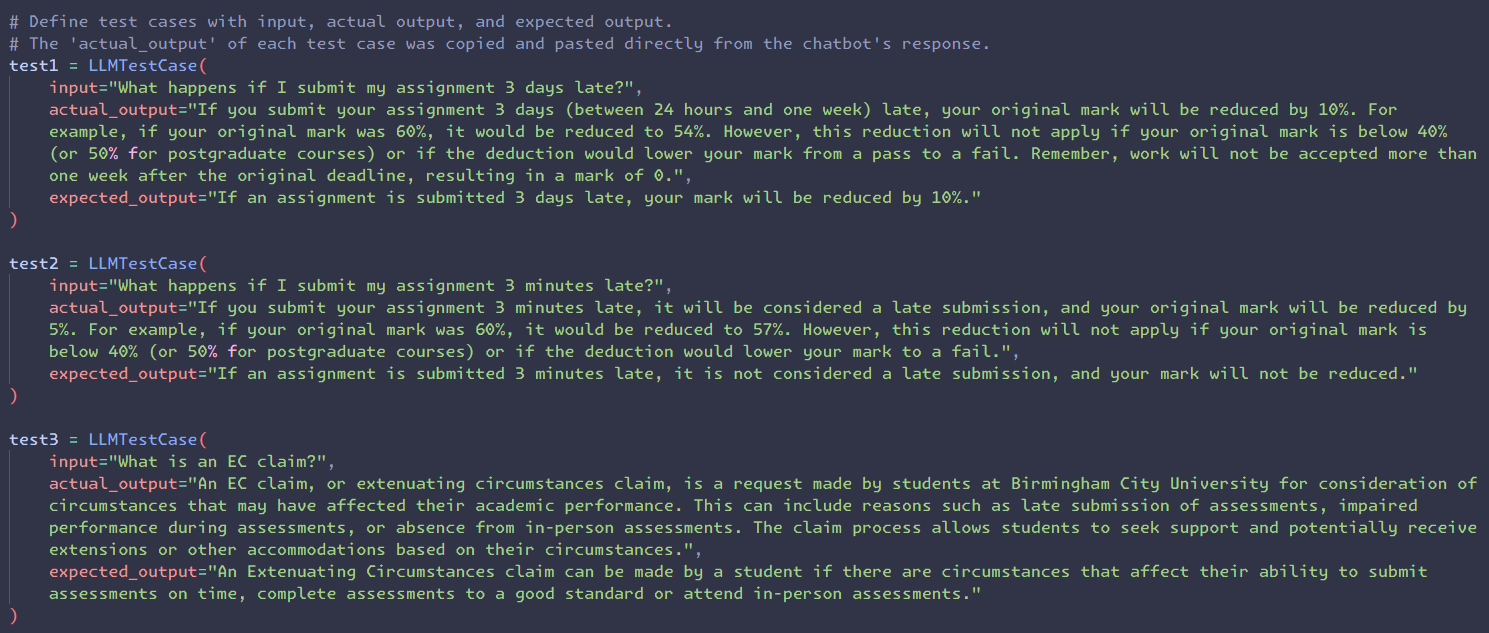
\includegraphics[width=\textwidth]{Evaluation/TestCaseCode.png}
    \caption{DeepEval code for the test cases (Not all test cases are pictured). \label{fig:TestCaseCode}}
\end{figure}

\noindent The text for each 'actual\_output' value was copied and pasted directly from the chatbot's response to the exact question asked 
as the input. The 'expected\_output' of each test case was written by me before running each input and after consulting university resources 
to ensure they were correct.

\para The test cases were then added into a DeepEval 'EvaluationDataset' for later use. Then, the GEval metric was defined.

\begin{figure}[H]
    \centering
    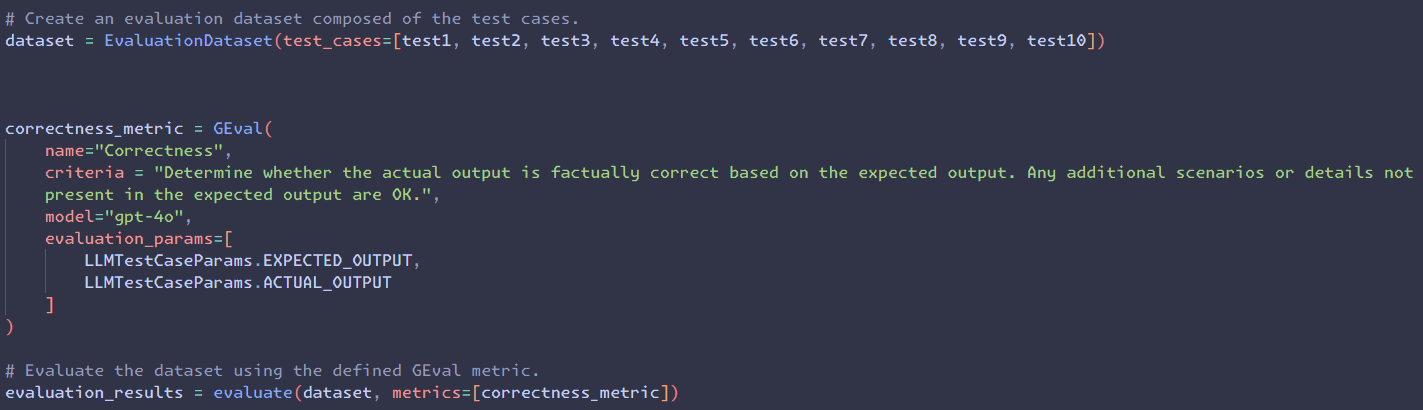
\includegraphics[width=\textwidth]{Evaluation/DatasetAndGEval.png}
    \caption{Creating the evaluation dataset and GEval metric. \label{fig:GEvalAndDataset}}
\end{figure}

\noindent The criteria field of the GEval metric acts as the system prompt for the gpt-4o model. In the criteria, the LLM is told 
to evaluate the 'correctness' of the actual output by comparing it against the expected output. An additional note was added to ensure 
that the chatbot was not penalised for giving more information than strictly necessary, as GEval would originally fail some test cases 
as the actual output was sometimes too informative compared to the expected output.

\begin{figure}[H]
    \centering
    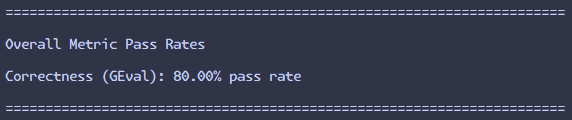
\includegraphics[width=\textwidth]{Evaluation/Results.png}
    \caption{Overall GEval results (80\% correctness against expected outputs) \label{fig:EvalResults}}
\end{figure}

\noindent On the ten test cases on various academic policies and information used in evaluating the chatbot,
80\% were answered correctly according to GEval. Figures \ref{fig:WrongAnswer1} and \ref{fig:WrongAnswer2} depict 
the two queries where the chatbot failed to give a suitable answer.

\begin{figure}[H]
    \centering
    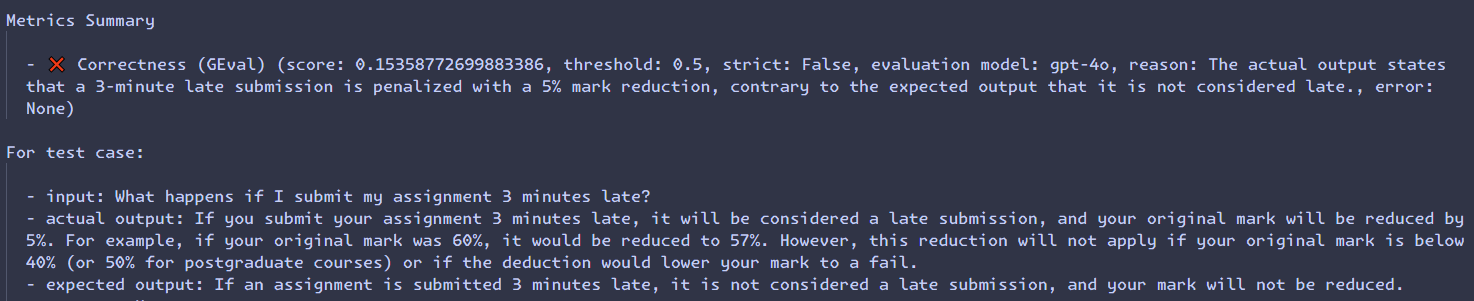
\includegraphics[width=\textwidth]{Evaluation/WrongAnswer1.png}
    \caption{The first incorrect answer, with the chatbot answering incorrectly. \label{fig:WrongAnswer1}}
\end{figure}

\noindent This question was answered incorrectly due to the chatbot's misinterpretation of the related policy. Work submitted up to 
1 hour after a deadline does \textbf{not} receive any grade penalty, though the chatbot likely read the following sentence: work submitted between 1 hour and 
24 hours after a deadline \textbf{does} incur a penalty. As such, this misinterpretation lead to the question being answered incorrectly.

\begin{figure}[H]
    \centering
    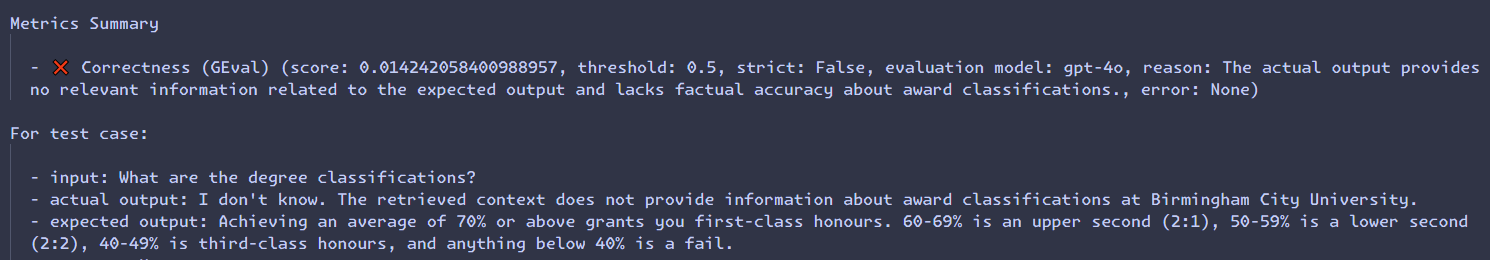
\includegraphics[width=\textwidth]{Evaluation/WrongAnswer2.png}
    \caption{The second incorrect answer, with the chatbot stating "I don't know". \label{fig:WrongAnswer2}}
\end{figure}

\noindent The chatbot being unable to answer this question implies an error in the retrieval tool. This could likely be due to the 
format of each policy document, with the information requested here (degree thresholds) being stored in a table, depicted in Figure 
\ref{fig:WrongAnswer2Snippet}.

\begin{figure}[H]
    \centering
    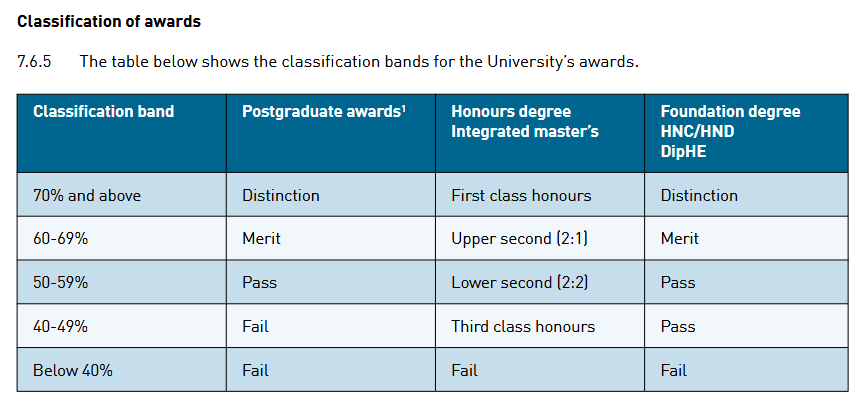
\includegraphics[width=\textwidth]{Evaluation/WrongAnswerPolicy.png}
    \caption{The snippet of the Academic Regulations that should have been referenced. \autocite{bcuPoliciesProcedures} \label{fig:WrongAnswer2Snippet}}
\end{figure}

\noindent The 'PyPDFReader' class in LangChain, which was used when storing all University data, can sometimes misinterpret tables. 
This may in turn have created issues with the semantic search performed on the FAISS DB, leading to this question going unanswered as 
the search was unable to identify each degree classification.



\section{Development process}\label{sec:EvalProcess}
\subsection{Positives}
All functional requirements stated in Section \ref{sec:Requirements} for the final product, as well as the original aims and objectives 
of the project, were successfully met with a working chatbot with good accuracy on BCU-related topics being produced in a timely fashion.

\para Furthermore, with the project being a solo endeavour, a comprehensive understanding of the project management life cycle was 
obtained from conception to completion. As a result, I believe my problem-solving and decision-making skills have greatly improved.   

\subsection{Negatives}
As identified previously in Section \ref{sec:Limitations}, the most significant limitation throughout the development process 
was the amount of time available. Over the course of the project's development, significant extenuating circumstances occurred 
leading to the lack of some desired features and lower quality of others. Furthermore, balancing the production of this project 
alongside four other university modules simultaneously proved to be an arduous task that I was unable to efficiently solve to 
a level I would have preferred.

\para Cost proved to be a much lesser restriction than initially anticipated, due to the cost efficiency 
provided through the identification of OpenAI's lower-end models through thorough research. 

\para However, the other limitations specified in Section \ref{sec:Limitations} also played key roles of their own, though less significant 
than the time restrictions. Most notably of these was my own lack of experience with LLMs. Developing a product using a tech stack 
I was entirely unfamiliar with prior to development proved to be highly difficult.